\chapter{Machine Learning Models}

\section{Introduction}
As explained in dept in the methodology chapter, the biometric data collected through the watches generated a total of 6 independent variables:

\begin{itemize}
    \item Heart Rate Maximum \textit{bm\_HR\_max}
    \item Heart Rate Average \textit{bm\_HR\_avg}
    \item Heart Rate Variability \textit{bm\_HR\_var}
    \item Activity Steps \textit{bm\_act\_steps}
    \item Sleep \textit{bm\_sleep}
\end{itemize}

The dependent variables that were collected through the gaming tests are:

\begin{itemize}
    \item Fine Motor Tracking Time \textit{fm\_avg\_trk\_time}
    \item Fine Motor Accuracy \textit{fm\_accuracy}
    \item Visual Average Response Time \textit{vx\_avg\_res\_time}
    \item Visual Shot Accuracy \textit{vx\_shot\_accuracy}
    \item Visual Target Accuracy \textit{vx\_trg\_accuracy}
    \item Audio Average Response Time \textit{au\_avg\_res\_time}
\end{itemize}

The goal based on the research question was to find the correlation between the independent and dependent variables. When approaching a machine learning problem, one of the fundamental
considerations is whether the problem is a regression or classification problem. 

\subsection*{Classification vs Regression Problem}
The main difference between a classification and regression problem is the type of dependent variable. The dependent variable is the variable that are being predicted. In 
classification, the dependent variable is categorical, meaning it can take one of a limited number of values. Examples includes predicting whether an email is spam or not,
predicting whether a patient has a disease or not. In regression, the dependent variable is continuous and numerical, meaning it can take any value within a range. Examples 
includes predicting house prices, stock prices, temperature. In this project, the dependent variables are continuous and numerical, making it a regression problem. The goal 
was to predict the dependent variables based on the biometric data collected from the watches. 

\section{Data Exploration}
The first step in the machine learning process was to explore the dataset. The dataset was loaded into a pandas dataframe and the first 5 rows were displayed to get an overview of the
data. The shape of the dataset was checked to see the number of rows and columns. The data types of the columns were checked to ensure that the data types were correct. The summary
statistics of the dataset were checked to analyze the min and max, mean, standard deviation, and median values of the dataset. The correlation between the independent and dependent
variables were checked to see if there was any correlation between the variables. the heatmap \ref{fig:correlation_heatmap} was then used to visualize the correlation between the variables. 

\begin{figure}[H]
    \centering
    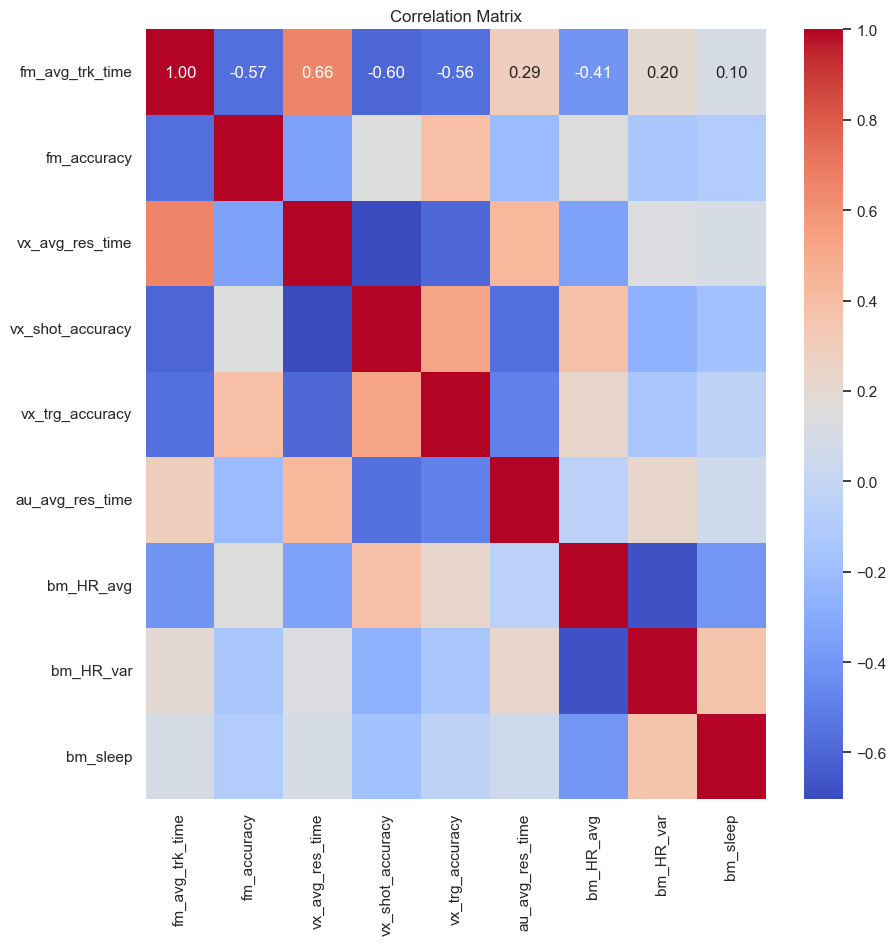
\includegraphics[width=1\textwidth]{images/correlation.png}
    \caption{Correlation Heatmap}
    \label{fig:correlation_heatmap}
\end{figure}

The analysis generated a correlation heatmap to explore the relationships between the features (independent variables) and the target variables (dependent variables).
It is a color-coded map, where the intensity of the color represents the strength of the correlation. With values that range from -1 to 1, where the negative values indicates a negative
correlation, positive values indicates a positive correlation and 0 indicates no correlation. The correlation heatmap provides a valuable insight into which features have the most 
significant influence on the target variables, helping understand the relationships within the data.

\subsubsection*{Heart Rate Average (\textit{bm\_HR\_avg})}
\begin{itemize}
    \item Fine Motor Tracking Time (\textit{fm\_avg\_trk\_time}): A negative correlation of \\ -0.41 suggests that as the average heart rate increases, the fine motor
    tracking time tasks decreases, indicating that individuals with faster heart rates tend to complete fine motor tasks a bit quicker.
    \item Fine Motor Accuracy (\textit{fm\_accuracy}): A positive correlation of 0.16 indicates a weak relationship suggesting that a higher heart rate average might be very 
    slightly associated with higher fine motor accuracy. It shows that there is a small tendency for individuals with a higher heart rate to be slightly more precise
    in tasks that need fine motor skills.
    \item Visual Average Response Time (\textit{vx\_avg\_res\_time}): A negative correlation of -0.35 suggests a moderate relationship where a higher average heart rate
    is associated with faster response times. It indicates that individuals with higher heart rates also tend to react faster to visual things.
    \item Visual Shot Accuracy (\textit{vx\_shot\_accuracy}): A positive correlation of 0.38 indicates a moderate relationship, suggesting that individuals with higher heart
    rate might have a better accuracy in shooting tasks.
    \item Visual Target Accuracy (\textit{vx\_trg\_accuracy}): A positive correlation of 0.22 indicates a weak relationship, suggesting that higher heart rates averages might
    be associated with slightly better visual target accuracy.
    \item Audio Average Response Time (\textit{au\_avg\_res\_time}): A very weak negative correlation of -0.05 suggest almost no relationship between average heart rate
    and audio response time. It indicates there is no real connection between heart rate and how quickly the individuals responds to sounds.
\end{itemize}

\subsubsection*{Hear Rate Variability (\textit{bm\_HR\_var})}

\begin{itemize}
    \item Fine Motor Tracking Time (\textit{fm\_avg\_trk\_time}): A positive correlation of 0.20 suggests a weak association where greater heart rate variability 
    might be associated with slightly longer fine motor tracking time tasks.
    
    \item Fine Motor Accuracy (\textit{fm\_accuracy}): A negative correlation of -0.14 suggest a very weak inverse relationship, where higher heart rate variability
    could be slightly associated with a decrease in fine motor accuracy.
    
    \item Visual Average Response Time (\textit{vx\_avg\_res\_time}): A positive correlation of 0.13 indicates very weak relationship, with slightly tendency for
    higher heart rate variability to be associated with longer visual response times. 
    
    \item Visual Shot Accuracy (\textit{vx\_shot\_accuracy}): A negative correlation of -0.27 indicates a weak to moderate inverse relationship, suggesting that
    higher rate variability might be associated with a decrease in visual shot accuracy. It suggests that individuals with higher heart rate variability might 
    have a lower accuracy in shooting tasks.
    
    \item Visual Target Accuracy (\textit{vx\_trg\_accuracy}): A negative correlation of -0.14 indicates a weak inverse relationship, suggesting that higher heart 
    variability could slightly correlate with lower visual target accuracy. It suggests that those with more variation in their heart rate might not be quite as good 
    at tasks that involve quickly identifying and selecting targets.
    
    \item Audio Average Response Time (\textit{au\_avg\_res\_time}): A positive correlation of 0.22 suggests a weak relationship, indicating that higher heart rate
    variability might be associated with slightly longer audio response times.
    
\end{itemize}


\subsubsection*{Sleep (\textit{bm\_sleep})}

\begin{itemize}
    \item Fine Motor Tracking Time (\textit{fm\_avg\_trk\_time}): A positive correlation of 0.10 suggests a very weak relationship, indicating that longer sleep duration
    may be very slightly correlated with longer fine motor tracking time. 
        
    \item Fine Motor Accuracy (\textit{fm\_accuracy}): With a value of -0.09, this negative correlation is very weak, indicating minimal inverse relationship between sleep
    and fine motor accuracy.
    
    \item Visual Average Response Time (\textit{vx\_avg\_res\_time}): At 0.10, the correlation is weak, suggesting a minimal tendency for more sleep to be associated with slightly
    longer response times in visual tasks.
    
    \item Visual Shot Accuracy (\textit{vx\_shot\_accuracy}): The value of -0.18 indicates a weak negative correlation, suggesting that increased sleep could be potentially be associated
    with a slight improvements in visual shot accuracy. 

    \item Visual Target Accuracy (\textit{vx\_trg\_accuracy}): At -0.04, the correlation is weak, indicating there is almost no relationship between sleep and visual target accuracy.
    
    \item Audio Average Response Time (\textit{au\_avg\_res\_time}): The correlation value of 0.06, which is very weak and suggests there is little to no meaningful correlation between
    sleep and response time to audio stimulus.
    
\end{itemize}


\section{Data Pre-processing}
The data underwent pre-processing to prepare it for machine learning models. This involved handling missing values by removing rows with missing entries as imputation wasn't possible.
Features like \textit{Activity Steps} and \textit{Heart Rate Maximum} were found to have outliers that were excluded from the data. 
To ensure all features contributed equally, the data was scaled using StandardScaler from the scikit-learn library. Irrelevant columns like \textit{\_id}, \textit{\_date} and 
\textit{\_user} were removed. Finally, the preprocessed data was split into training (80\%) and testing (20\%) sets. The independent variables (features) were separated into
X (independent), and the dependent variable (target) into a y. This prepared the data for use in machine learning models.


\section{Model Selection and Evaluation}
Various machine learning models were explored to address the research question and predict the dependent variables based on the collected biometric and gaming test. Each team member
focused on developing and evaluating a model to achieve the best predictive performance. 

\subsection{Classical ML Regression Models}
The classical machine learning regression models were explored to predict the dependent variables based on the independent variables. 
The training process involved fitting the models on the training dataset and then assessing their performance on the unseen testing dataset. Mean squared error (MSE) served as the evaluation metric,
with the model achieving the lowest MSE being chosen as the best performing model for further analysis. This approach ensures the chosen model generalizes well to unseen data, avoiding
overfitting to the training set. The following algorithm were explored:

\begin{itemize}
    \item Linear Regression: Chose as a baseline for its simplicity and Interpretability, assuming a linear relationship between the dependent and independent variables.
    \item Random Forest Regressor: Chose for its ability to capture complex non-linear relationships in the data and its robustness to overfitting.
    \item Support Vector Regressor: It was chosen for its ability to capture complex relationships in the data and its robustness to outliers.
    \item K-Nearest Neighbours Regressor: Chose for its simplicity and effectiveness in regression tasks, making predictions based on the average of the k-nearest neighbours in the feature space.
\end{itemize}

Once the best performing model for each dependent variable was selected, the model was then evaluated using the testing dataset and actual versus predicted values were plotted to see
how well the model performed. 

\subsection{Actual vs Predicted Analysis}
The actual versus predicted plot was used to visualize how well the model performed. The actual values were plotted against the predicted values to see how well the model predicted the
dependent variables. The plot was used to see if the model was underfitting or overfitting the data. If the points were close to the line, it indicated that the model was performing well.
If the points were scattered, it indicated that the model was not performing well. The plot was used to see if the model was capturing the underlying patterns in the data. Below are the 
actual versus predicted plots for the best performing model for each dependent variable.

\subsection*{Fine Motor Tracking Time}

\begin{figure}[htbp]
    \centering
    \begin{subfigure}[b]{0.49\textwidth}
        \centering
        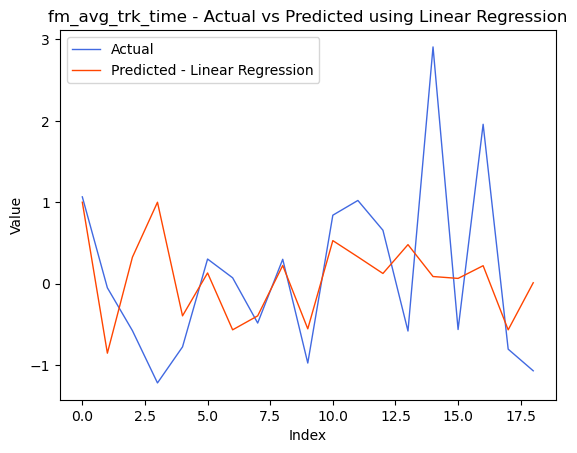
\includegraphics[width=\textwidth]{images/regressionCharts/test_data_fine_motor_tracking_time.png}
        \caption{Actual vs Predicted (Test Data)}
        \label{fig:actual_vs_predicted_fm_avg_trk_time_test}
    \end{subfigure}\hfill
    \begin{subfigure}[b]{0.49\textwidth}
        \centering
        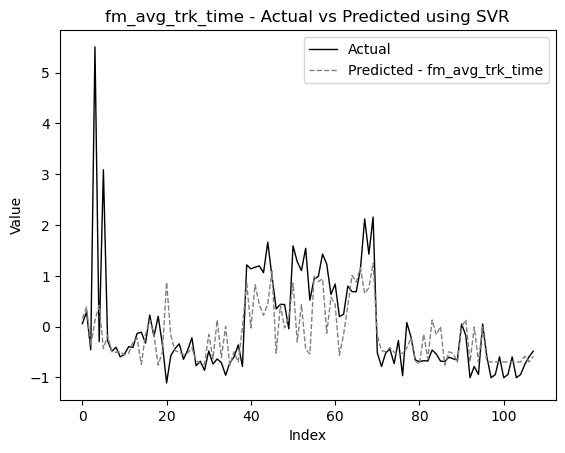
\includegraphics[width=\textwidth]{images/regressionCharts/all_data_fine_motor_tracking_time.png}
        \caption{Actual vs Predicted (All Data)}
        \label{fig:actual_vs_predicted_fm_avg_trk_time_all_data}
    \end{subfigure}
    \caption{Fine Motor Tracking Time Actual vs Predicted}
    \label{fig:fine_motor_tracking_time_comparison}
\end{figure}

\subsubsection*{Test Data Evaluation}

\begin{itemize}
    \item \textbf{Trend}: Figure \ref{fig:actual_vs_predicted_fm_avg_trk_time_test} shows the actual versus predicted values for the Fine Motor Average Tracking Time using the test data. The model that performed 
    the best for this dependent variable was the Linear Regression Model. The model's predictions generally matched the direction of the actual test data's trend. The peaks and troughs of the
    actual data were also found in the predicted data, with some deviations. 
    \item \textbf{Variance}: There is a noticeable variance between the actual and predicted values, specially at the extremes. For instance, the model appears to underestimate the highest values
    and overestimate the lowest values.
    \item \textbf{Consistency}: The model shows decent consistency when the actual values are around the mean but is less consistent at capturing sudden changes in the actual data, such as sharp spikes ot dips.
\end{itemize}

\subsubsection*{All Data Evaluation}

\begin{itemize}
    \item \textbf{Trend}: Figure \ref{fig:actual_vs_predicted_fm_avg_trk_time_all_data} shows the actual versus predicted values for the Fine Motor Average Tracking Time using all the data
    available. When evaluating all the data, the model predictions closely follow the actual data's trend. This indicates that the model has learned the overall behavior of the dataset quite well.
    Similar to the test data, the model captures the general pattern of movement in the actual values, but might not always match the amplitude of changes.
    \item \textbf{Variance}: The variance between the actual and predicted values over all the data seems to be lower compared to the test data. This suggests that the model has been 
    effectively trained to understand the data as a whole. Some exceptions occur where the actual values show significant deviation from the mean. In these areas, the predictions do not fully 
    capture the extent of the actual values and show some deviation.
    \item \textbf{Consistency}: The model shows good consistency in predicting the values when the actual values are around the mean. The predictions often match the actual values quite closely.
\end{itemize}

Overall the Linear Regression Model performed well in both scenarios, capturing the general trends of the Fine Motor Tracking Time and showing good consistency in prediction.
The model, however, seems to struggle with accurately predicting the more extreme values in the dataset. It highlights the need for improving the model's performance on the more complex
or extreme segments of the data.

\subsection*{Fine Motor Accuracy}

\begin{figure}[htbp]
    \centering
    \begin{subfigure}[b]{0.49\textwidth}
        \centering
        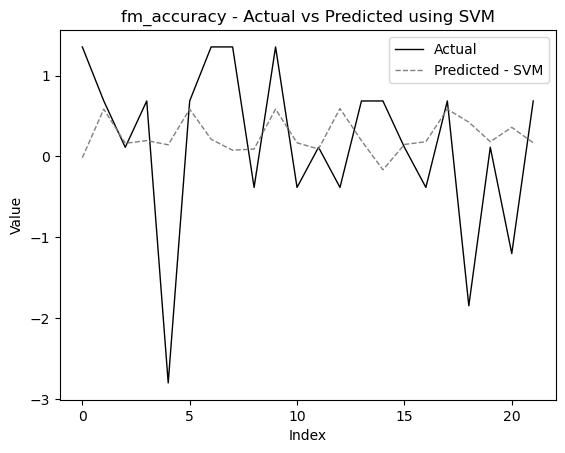
\includegraphics[width=\textwidth]{images/regressionCharts/test_data_fine_motor_accuracy.png}
        \caption{Actual vs Predicted (Test Data)}
        \label{fig:actual_vs_predicted_fm_accuracy_test}
    \end{subfigure}\hfill
    \begin{subfigure}[b]{0.49\textwidth}
        \centering
        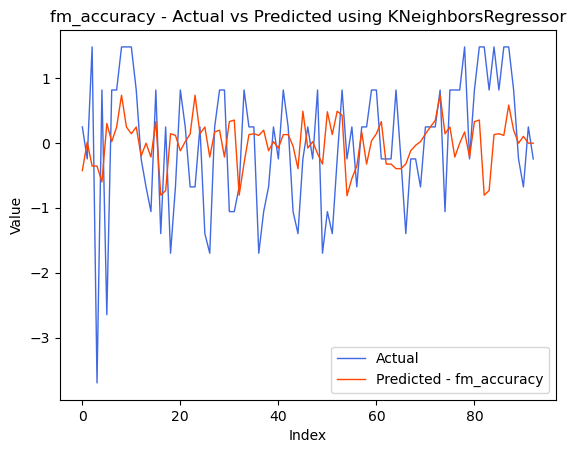
\includegraphics[width=\textwidth]{images/regressionCharts/all_data_fine_motor_accuracy.png}
        \caption{Actual vs Predicted (All Data)}
        \label{fig:actual_vs_predicted_fm_accuracy_all_data}
    \end{subfigure}
    \caption{Fine Motor Accuracy Actual vs Predicted}
    \label{fig:fine_motor_accuracy_comparison}
\end{figure}

\subsubsection*{Test Data Evaluation}

\begin{itemize}
    \item \textbf{Trend}: Figure \ref{fig:actual_vs_predicted_fm_accuracy_test} shows the actual versus predicted values for the Fine Motor Accuracy using the test data. The model 
    that performed the best for this dependent variable was the k-Nearest Neighbors Regressor. The model appears to capture the general trend of the actual data. It follows the directional
    changes, going up and down as the actual values do, but not with perfect alignment.
    \item \textbf{Variance}: There is a noticeable variance between the actual and predicted values, especially at the extremes. While the model tends to underpredict some of the sharper
    declines in actual values, it still remains relatively closely to the true data points.
    \item \textbf{Consistency}: There is a moderate level of consistency in the predictions. The model seems to perform well when the actual values are not showing extreme behavior. However,
    in instances where the actual values show sharp changes, the model's consistency is reduced.
\end{itemize}

\subsubsection*{All Data Evaluation}

\begin{itemize}
    \item \textbf{Trend}: Figure \ref{fig:actual_vs_predicted_fm_accuracy_all_data} shows the actual versus predicted values for the Fine Motor Accuracy using all the data available. 
    Across the full dataset, the k-Nearest Neighbors Regressor model generally traces the movements of the actual values well. This suggests a solid understanding of the underlying patterns
    in the full range of data. Despite some misalignment, the predicted values consistently mirror the ups and downs in the actual data, indicating the model's capability to track the 
    overall trend.
    \item \textbf{Variance}: Compared to the test data, the variance in the full data set appears to slightly more visible. The predictions occasionally deviate significantly from the
    actual values, particularly where there are sharp changes in the actual data or outliers in the actual data.
    \item \textbf{Consistency}: The model shows good consistency in predicting the values when the actual values are around the mean. It does, however, display some inconsistencies, again
    mainly where there are larger deviations in the actual data.    
\end{itemize}

Overall, the k-Nearest Neighbors Regressor model demonstrated an ability to capture the general trends in the Fine Motor Accuracy both in the test set and the full dataset. While the model tends
to stay close to the actual values, it does show some variance and inconsistency, particularly in areas where the actual data shows sharp changes or outliers. This suggests that the
model may need further refinement to improve its performance in these more complex or extreme segments of the data. Also, the model may benefit from more data to help it better understand
the full range of patterns in the dataset.

\subsection*{Visual Average Response Time}

\begin{figure}[htbp]
    \centering
    \begin{subfigure}[b]{0.49\textwidth}
        \centering
        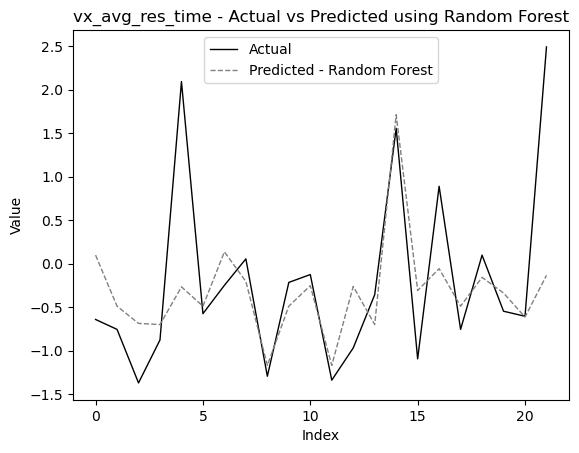
\includegraphics[width=\textwidth]{images/regressionCharts/test_data_visual_average_response_time.png}
        \caption{Actual vs Predicted (Test Data)}
        \label{fig:actual_vs_predicted_vx_avg_res_time_test}
    \end{subfigure}\hfill
    \begin{subfigure}[b]{0.49\textwidth}
        \centering
        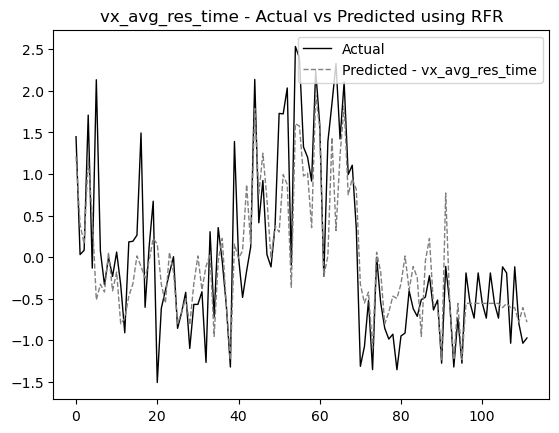
\includegraphics[width=\textwidth]{images/regressionCharts/all_data_visual_average_response_time.png}
        \caption{Actual vs Predicted (All Data)}
        \label{fig:actual_vs_predicted_vx_avg_res_time_all_data}
    \end{subfigure}
    \caption{Visual Average Response Time Actual vs Predicted}
    \label{fig:visual_avg_response_time_comparison}
\end{figure}

\subsubsection*{Test Data Evaluation}

\begin{itemize}
    \item \textbf{Trend}: Figure \ref{fig:actual_vs_predicted_vx_avg_res_time_test} shows the actual versus predicted values for the Visual Average Response Time using the test data. 
    The model that performed the best for this dependent variable was the k-Nearest Neighbors Regressor. The model successfully captured the underlying trend of the actual data. The predicted line reflects the high and low points of the actual data, demonstrating the model's ability 
    to learn the fundamental patterns in the data.
    \item \textbf{Variance}: While the model generally aligns with the actual values, there are instances where the predicted values deviate from the actual data. Specifically, the model doesn't
    always capture the sharpness and valleys which can be seen in several areas of the actual data.
    \item \textbf{Consistency}: In sections where the data does not fluctuate significantly, the model's predictions are quite stable and track the actual data closely. This suggests a level
    of reliability in the model's predictions under more controlled variations in the response time.
\end{itemize}

\subsubsection*{All Data Evaluation}

\begin{itemize}
    \item \textbf{Trend}: Figure \ref{fig:actual_vs_predicted_vx_avg_res_time_all_data} shows the actual versus predicted values for the Visual Average Response Time using all the data available
    When applied to the entire dataset, the model displays an ability to mimic the overall trend line of the actual data. The predictions fluctuate in line with the actual values, 
    showing an understanding of the larger patterns in the data.    
    \item \textbf{Variance}: As with the test data, there are discrepancies between the actual and predicted values; these are most apparent where is a sharp change in the actual data.
    The model sometimes smooths out these abrupt changes, leading to a slight deviation from the actual values.    
    \item \textbf{Consistency}: The model shows a decent level of consistency throughout the entire data range. While there are mismatches, particularly in areas of high variability,
    the model maintains a close following with the actual values for the most part.
\end{itemize}

In both the test data and the full dataset, the k-Nearest Neighbors Regressor model for the Visual Average Response Time demonstrates effectiveness in capturing the main trends and movements.
It shows a good degree of consistency, with understandable variance in places where the data is more complex or extreme. The model appears to perform better when dealing with average levels of 
fluctuation but might require further tuning to more accurately predict the more extreme variations observed in the actual data.


\subsection*{Visual Shot Accuracy}

\begin{figure}[htbp]
    \centering
    \begin{subfigure}[b]{0.49\textwidth}
        \centering
        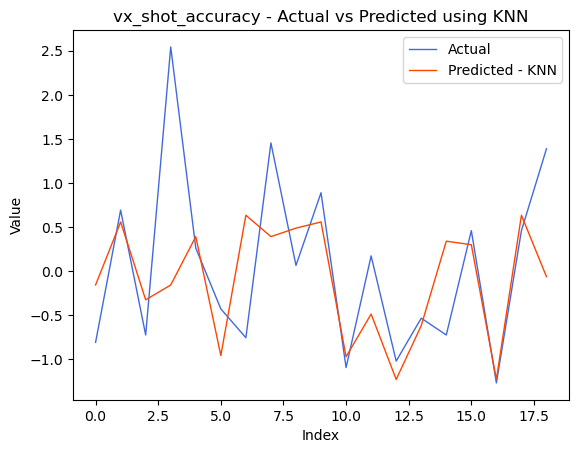
\includegraphics[width=\textwidth]{images/regressionCharts/test_data_visual_shot_accuracy.png}
        \caption{Actual vs Predicted (Test Data)}
        \label{fig:actual_vs_predicted_vx_shot_accuracy_test}
    \end{subfigure}\hfill
    \begin{subfigure}[b]{0.49\textwidth}
        \centering
        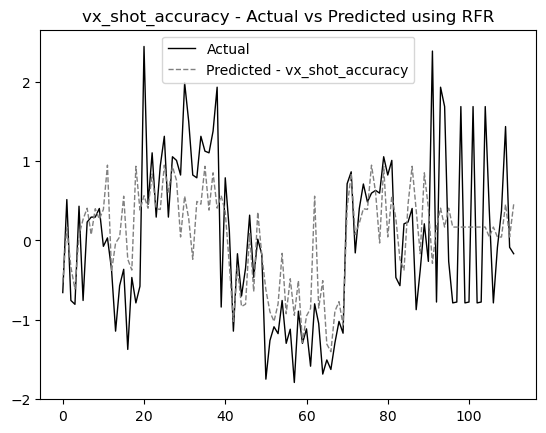
\includegraphics[width=\textwidth]{images/regressionCharts/all_data_visual_shot_accuracy.png}
        \caption{Actual vs Predicted (All Data)}
        \label{fig:actual_vs_predicted_vx_shot_accuracy_all_data}
    \end{subfigure}
    \caption{Visual Shot Accuracy Actual vs Predicted}
    \label{fig:visual_shot_accuracy_comparison}
\end{figure}

\subsubsection*{Test Data Evaluation}

\begin{itemize}
    \item \textbf{Trend}: Figure \ref{fig:actual_vs_predicted_vx_shot_accuracy_test} shows the actual versus predicted values for the Visual Shot Accuracy using the test data. The model that performed 
    the best for this dependent variable was the k-Nearest Neighbors Regressor. The KNN model seems to reasonably follow the general of the actual values. It responds to the directional shifts in the data,
    rising and falling in correlation with the actual data. However, there are noticeable disparities at certain points, indicating that while the model detects the overall pattern, it does not always align
    perfectly with the actual data's trajectory.       
    \item \textbf{Variance}: The variance between the predicted and actual values is visible. Particularly at peaks the model's predicted values appear to underestimate the actual values. The model performs 
    more reliably at data points that are closer to the central trend and shows more deviation at the extremes.    
    \item \textbf{Consistency}: The KNN models demonstrates moderate consistency throughout the test dataset, capturing the general trend of the actual data with some fidelity. However, its ability to 
    mirror the actual data precisely at every point is limited, especially where there is significant fluctuation in the actual data.
    
\end{itemize}

\subsubsection*{All Data Evaluation}

\begin{itemize}
    \item \textbf{Trend}: Figure \ref{fig:actual_vs_predicted_vx_shot_accuracy_all_data} shows the actual versus predicted values for the Visual Shot Accuracy using all the data available.  
    With the entire dataset, the KNN model's prediction still follow the actual values' general trend, suggesting an understanding of the global behavior of the data. The model struggles
    with sharp spikes and drops, smoothing over some of the more extreme changes in the actual data. 
    
    \item \textbf{Variance}: The variance across the full dataset seems to be slightly more controlled than in the test data, although discrepancies remain. The model does not perfectly capture
    the amplitude of changes, particularly the higher peaks and lower troughs in the actual data.
    
    \item \textbf{Consistency}: Across the full scope of data, the KNN model's predictions display an adequate level of consistency, reflecting a steady predictive performance that often aligns well with the real values.
    However, the model's prediction can diverge from the actual data at points, indicating room for improvement in model accuracy.
    
\end{itemize}

The k-Nearest Neighbors Regressor model shows that it captured the central tendencies and fluctuations in Visual Shot Accuracy both in the testing phase and across the complete dataset. The model's capability of 
following the trends is a strong point, but its prediction variance and the consistency of its performance present areas for improvement. 


\subsection*{Visual Target Accuracy}

\begin{figure}[htbp]
    \centering
    \begin{subfigure}[b]{0.49\textwidth}
        \centering
        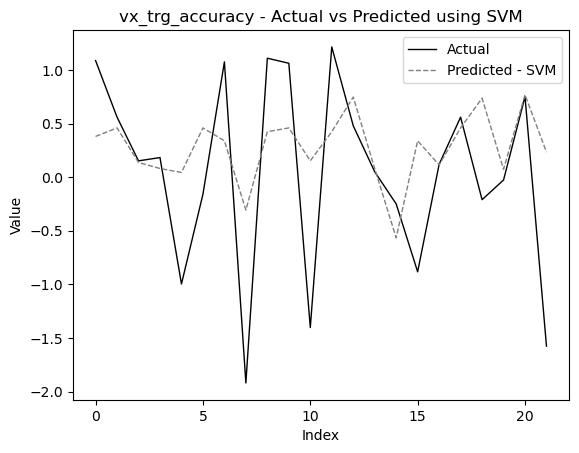
\includegraphics[width=\textwidth]{images/regressionCharts/test_data_visual_target_accuracy.png}
        \caption{Actual vs Predicted (Test Data)}
        \label{fig:actual_vs_predicted_vx_trg_accuracy_test}
    \end{subfigure}\hfill
    \begin{subfigure}[b]{0.49\textwidth}
        \centering
        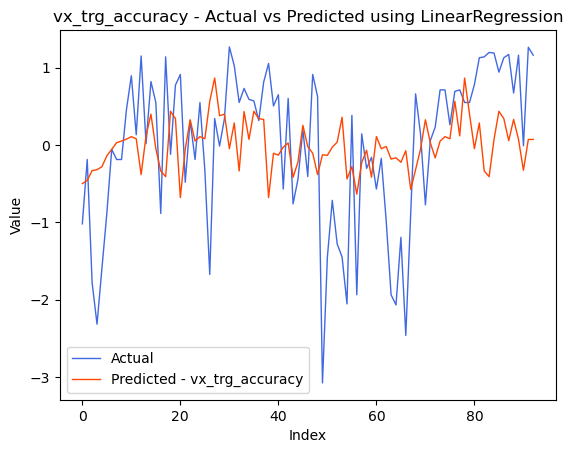
\includegraphics[width=\textwidth]{images/regressionCharts/all_data_visual_target_accuracy.png}
        \caption{Actual vs Predicted (All Data)}
        \label{fig:actual_vs_predicted_vx_trg_accuracy_all_data}
    \end{subfigure}
    \caption{Visual Target Accuracy Actual vs Predicted}
    \label{fig:visual_target_accuracy_comparison}
\end{figure}

\subsubsection*{Test Data Evaluation}

\begin{itemize}
    \item \textbf{Trend}: Figure \ref{fig:actual_vs_predicted_vx_trg_accuracy_test} shows the actual versus predicted values for the Visual Target Accuracy using the test data. The model that performed
    best for this dependent variable was the Linear Regression Model. The model's predicted outcomes show a basic alignment with the actual data's trend. The general ups and downs in the actual data are
    mirrored in the model's predictions, indicating a broad understanding of the data's patterns. However, there are instances where the model does not perfectly trace the actual data's peaks and troughs, 
    suggesting that while the trend is recognized, the precision of the model could be improved.

    \item \textbf{Variance}: The variance between the actual and predicted values seems moderate. The model seems to smooth out some of the actual data fluctuations, not capturing the extremes as it should.
        
    \item \textbf{Consistency}: The model maintains a fair level of consistency across the test dataset. The predicted values are regularly close to the actual data, although they do not consistently match the
    actual values with high fidelity. 
    
\end{itemize}

\subsubsection*{All Data Evaluation}

\begin{itemize}
    \item \textbf{Trend}: Figure \ref{fig:actual_vs_predicted_vx_trg_accuracy_all_data} shows the actual versus predicted values for the Visual Target Accuracy using all the data available. Over the entire dataset,
    the Linear Regression Model's predictions generally follow the trend of the actual values, indicating a stable understanding of the data's patterns. Similar to the test data, the predictions are in line with the
    overall movements but occasionally miss the mark in capturing the specific oscillations in the actual data.
    
    \item \textbf{Variance}: The prediction variance across the full dataset appears somewhat greater compared to the test data. This could be due to the inclusion of more diverse data points, revealing the model's 
    limitations in adapting to broader patterns. The model especially tends to underpredict some of the lower values, leading to a noticeable deviation in the more extreme data points.
    
    \item \textbf{Consistency}: Throughout the full dataset, the consistency of the model's predictions is apparent but not without error. The model seems to stay true to the mean trajectory but lacks in tracking the 
    finer details of the actual data. 
        
\end{itemize}

The Linear Regression Model for the Visual Target Accuracy demonstrates a basic understanding of the data's patterns, capturing the general trends in the test data and the full dataset. However, the model exhibits
a level of variance that indicates room for improvement in its predictive accuracy. Specifically, the model could benefit from refinement to better capture the more extreme values in the actual data.

\subsection*{Audio Average Response Time}

\begin{figure}[htbp]
    \centering
    \begin{subfigure}[b]{0.49\textwidth}
        \centering
        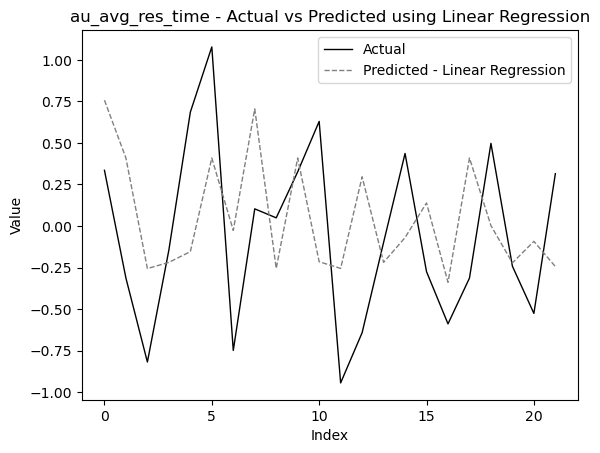
\includegraphics[width=\textwidth]{images/regressionCharts/test_data_audio_average_response_time.png}
        \caption{Actual vs Predicted (Test Data)}
        \label{fig:actual_vs_predicted_au_avg_res_time_test}
    \end{subfigure}\hfill
    \begin{subfigure}[b]{0.49\textwidth}
        \centering
        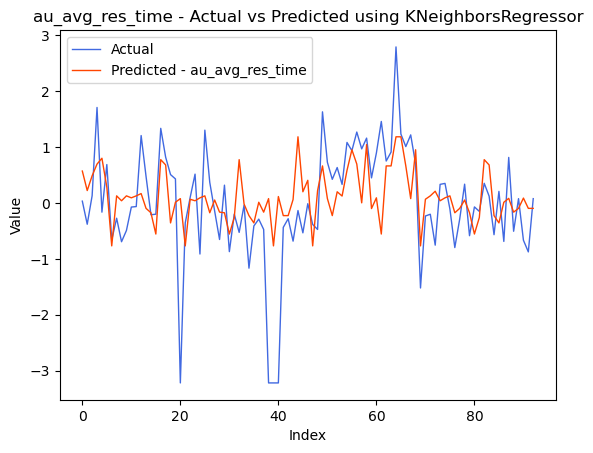
\includegraphics[width=\textwidth]{images/regressionCharts/all_data_audio_average_response_time.png}
        \caption{Actual vs Predicted (All Data)}
        \label{fig:actual_vs_predicted_au_avg_res_time_all_data}
    \end{subfigure}
    \caption{Audio Average Response Time Actual vs Predicted}
    \label{fig:audio_avg_response_time_comparison}
\end{figure}

\subsubsection*{Test Data Evaluation}

\begin{itemize}
    \item \textbf{Trend}: Figure \ref{fig:actual_vs_predicted_au_avg_res_time_test} shows the actual versus predicted values for the Audio Average Response Time using the test data. The model that performed
    best for this dependent variable was the k-Nearest Neighbors Regressor. The model's predictions tends to reflect the actual data's trend, indicating a general grasp of the data's patterns. The prediction line shows 
    a consistent rise and fall pattern that corresponds with the actual data line, illustrating the model's ability to track changes in response time.    
    
    \item \textbf{Variance}: There is a noticeable divergence between the predicted and actual values at several points across the dataset. This variance highlights areas where the model's predictions are not 
    as close to the actual values, especially at sharp downward and upward turns in the actual data.    
    
    \item \textbf{Consistency}: Despite some variances, the KNN model remains fairly consistent in its predictions across throughout the test dataset. While it does not precisely match the actual values, it provides 
    a reasonably consistent estimation, particularly in the middle range of the response time values.

\end{itemize}


\subsubsection*{All Data Evaluation}

\begin{itemize}
    \item \textbf{Trend}: Figure \ref{fig:actual_vs_predicted_au_avg_res_time_all_data} shows the actual versus predicted values for the Audio Average Response Time using all the data available. Looking
    at the entire dataset, the KNN model again mirrors the general trend of the actual data, showing an ability to comprehend the ups and downs in the response time. It captures the global trend across a 
    broader range of data points.    
    
    \item \textbf{Variance}: The overall variance in predictions across the entire dataset appears to be somewhat controlled, but deviations are still present. The model occasionally smoothens the extremities 
    in the actual data, leading under or overestimation in some segments.
    
    \item \textbf{Consistency}: In terms of consistency, the model show a reasonable degree of reliability across the entire dataset. Its predictions are in alignment with the direction of the actual data,
    even though it does not match every peak and valley with precision.
    
\end{itemize}


The k-Nearest Neighbors Regressor model for the Audio Average Response Time demonstrates a competent understanding of the Audio Average Response Time patterns, both in the test and the full dataset. It demonstrates 
a level of consistency that suggests it captures the variable's fundamental characteristics. However, the model's prediction exhibit some variance, indicating room for improvement in its ability to capture more
subtle fluctuations in the data.


\section{Neural Network Regression Model}


